\documentclass{article}
\usepackage{amsmath}
\usepackage{graphicx}
\usepackage[utf8]{inputenc}
\usepackage{parskip}%

\setcounter{secnumdepth}{0}

\date{}
\author{Kaan Aksoy | Feb 13, 2020}

\begin{document}

\maketitle

\section{Coin in Square}

We would like to compute the probability of a $3/4$-inch 
diameter coin landing on a table covered by a grid of $1$ 
by $1$ inch squares without touching the edges of any square.

\begin{figure}[h]
\centering
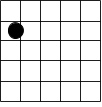
\includegraphics{CoinOnGrid}
\caption{Coin landing on an edge of the square grid}
\end{figure}

To calculate this probability, consider a single square 
on the grid. Then, consider the center of the landed coin 
as a point in that square. In order for the coin to not be 
touching the square, the center of the coin must be 
within a $1/4$ by $1/4$ area at the center of the square:

\begin{figure}[h]
    \centering
    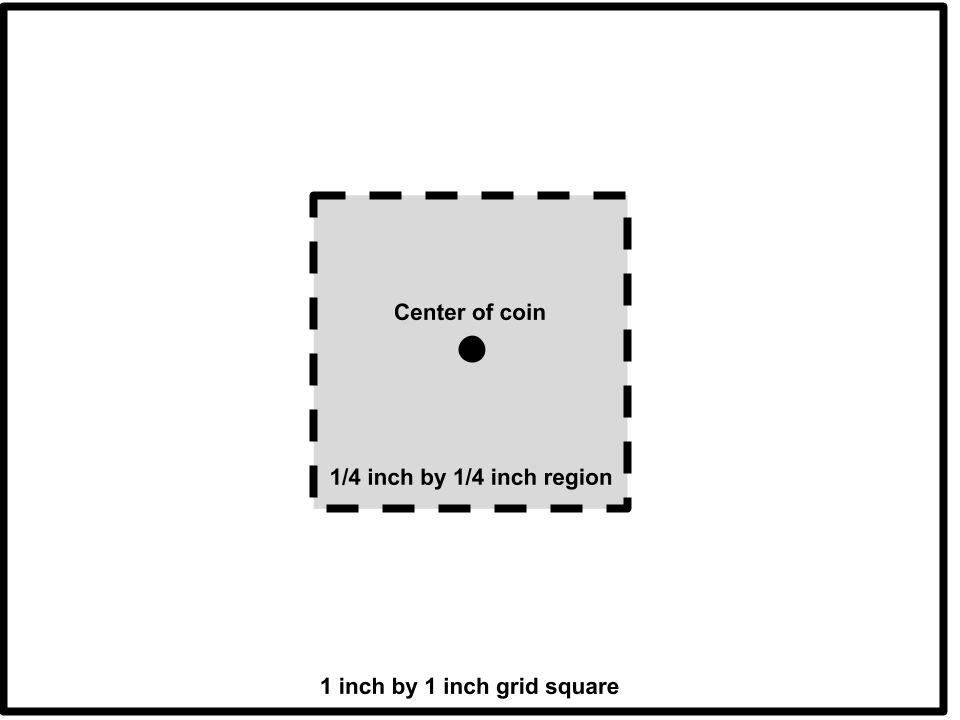
\includegraphics[width=6.25cm]{CoinValidSpots}
    \caption{Caption}
\end{figure}

Thus, for one grid square, the probability of the 
coin not touching an edge is:

$$ \frac{\left( \frac{1}{4} \right)^2}{(1)^2} = \frac{1}{16}$$

When considering an arbitrarily large grid, this probability 
remains the same, since adding more squares to the 
grid does not affect the overall proportion of places the coin 
can land without touching an edge. Thus, the final answer is $\frac{1}{16}$.

\end{document}